\documentclass[11pt,twocolumn]{article}
\usepackage[left=1.5cm,right=1.5cm,top=2cm,bottom=2cm]{geometry}
\usepackage{amsfonts}
\usepackage{amsmath}
\usepackage{graphicx}
\usepackage{hyperref}
\hypersetup{
    % hidelinks
    colorlinks=true,
    linkcolor=blue,
    filecolor=magenta,      
    urlcolor=cyan,
    pdftitle={Sharelatex Example},
    bookmarks=true,
    pdfpagemode=FullScreen,
}
\usepackage{cleveref}
\usepackage{float}
% \usepackage{caption}
\usepackage{subcaption}

\usepackage[ruled,vlined]{algorithm2e}
\usepackage[noend]{algpseudocode}


\title{HAL Matrix}
\author{Rishitosh Kumar Singh}

\begin{document}
\maketitle

\section{Problem}
    Consider a matrix $A$ of size $\mathbb{R}^{nd \times nd}$, where each non-overlapping $d \times d$ block of the matrix, $D_{ij}$ , is a diagonal matrix. So the matrix consists of $n^2$ such blocks. An example of such a matrix is shown below:
    \begin{equation}
        \nonumber
        \begin{bmatrix} D_{11} & D_{12} & D_{13} & \cdots & D_{1n} \\ D_{21} & D_{22} & D_{23} & \cdots & D_{2n} \\ \cdots & \cdots & \cdots & \cdots & \cdots \\ D_{n1} & D_{n2} & D_{n3} & \cdots & D_{nn} \end{bmatrix}
    \end{equation}

    Construct an efficient data structure to reploopresent such matrices and devise algorithms to perform matrix operations, such as matrix multiplications and matrix inverse, on the data structure you designed. Provide a technical write-up of your solution along with associated code implementing your solution.

\section{Solution}
    
    Data Structure to save matrix stated in the problem statement must be memory efficient and should be compatible with various matrix operations. It can be observed in \cref{img:matrix} that due to presence of block diagonal matrix $D_{ij}$, the final matrix $A$ can be treated as a sparse matrix if, $d \neq 1$. So, instead of saving all $nd \times nd$ elements, only $nd$ elements need to be saved, thus reducing memory requirement by $\frac{1}{d}$ factor.

    \begin{figure}[H]
        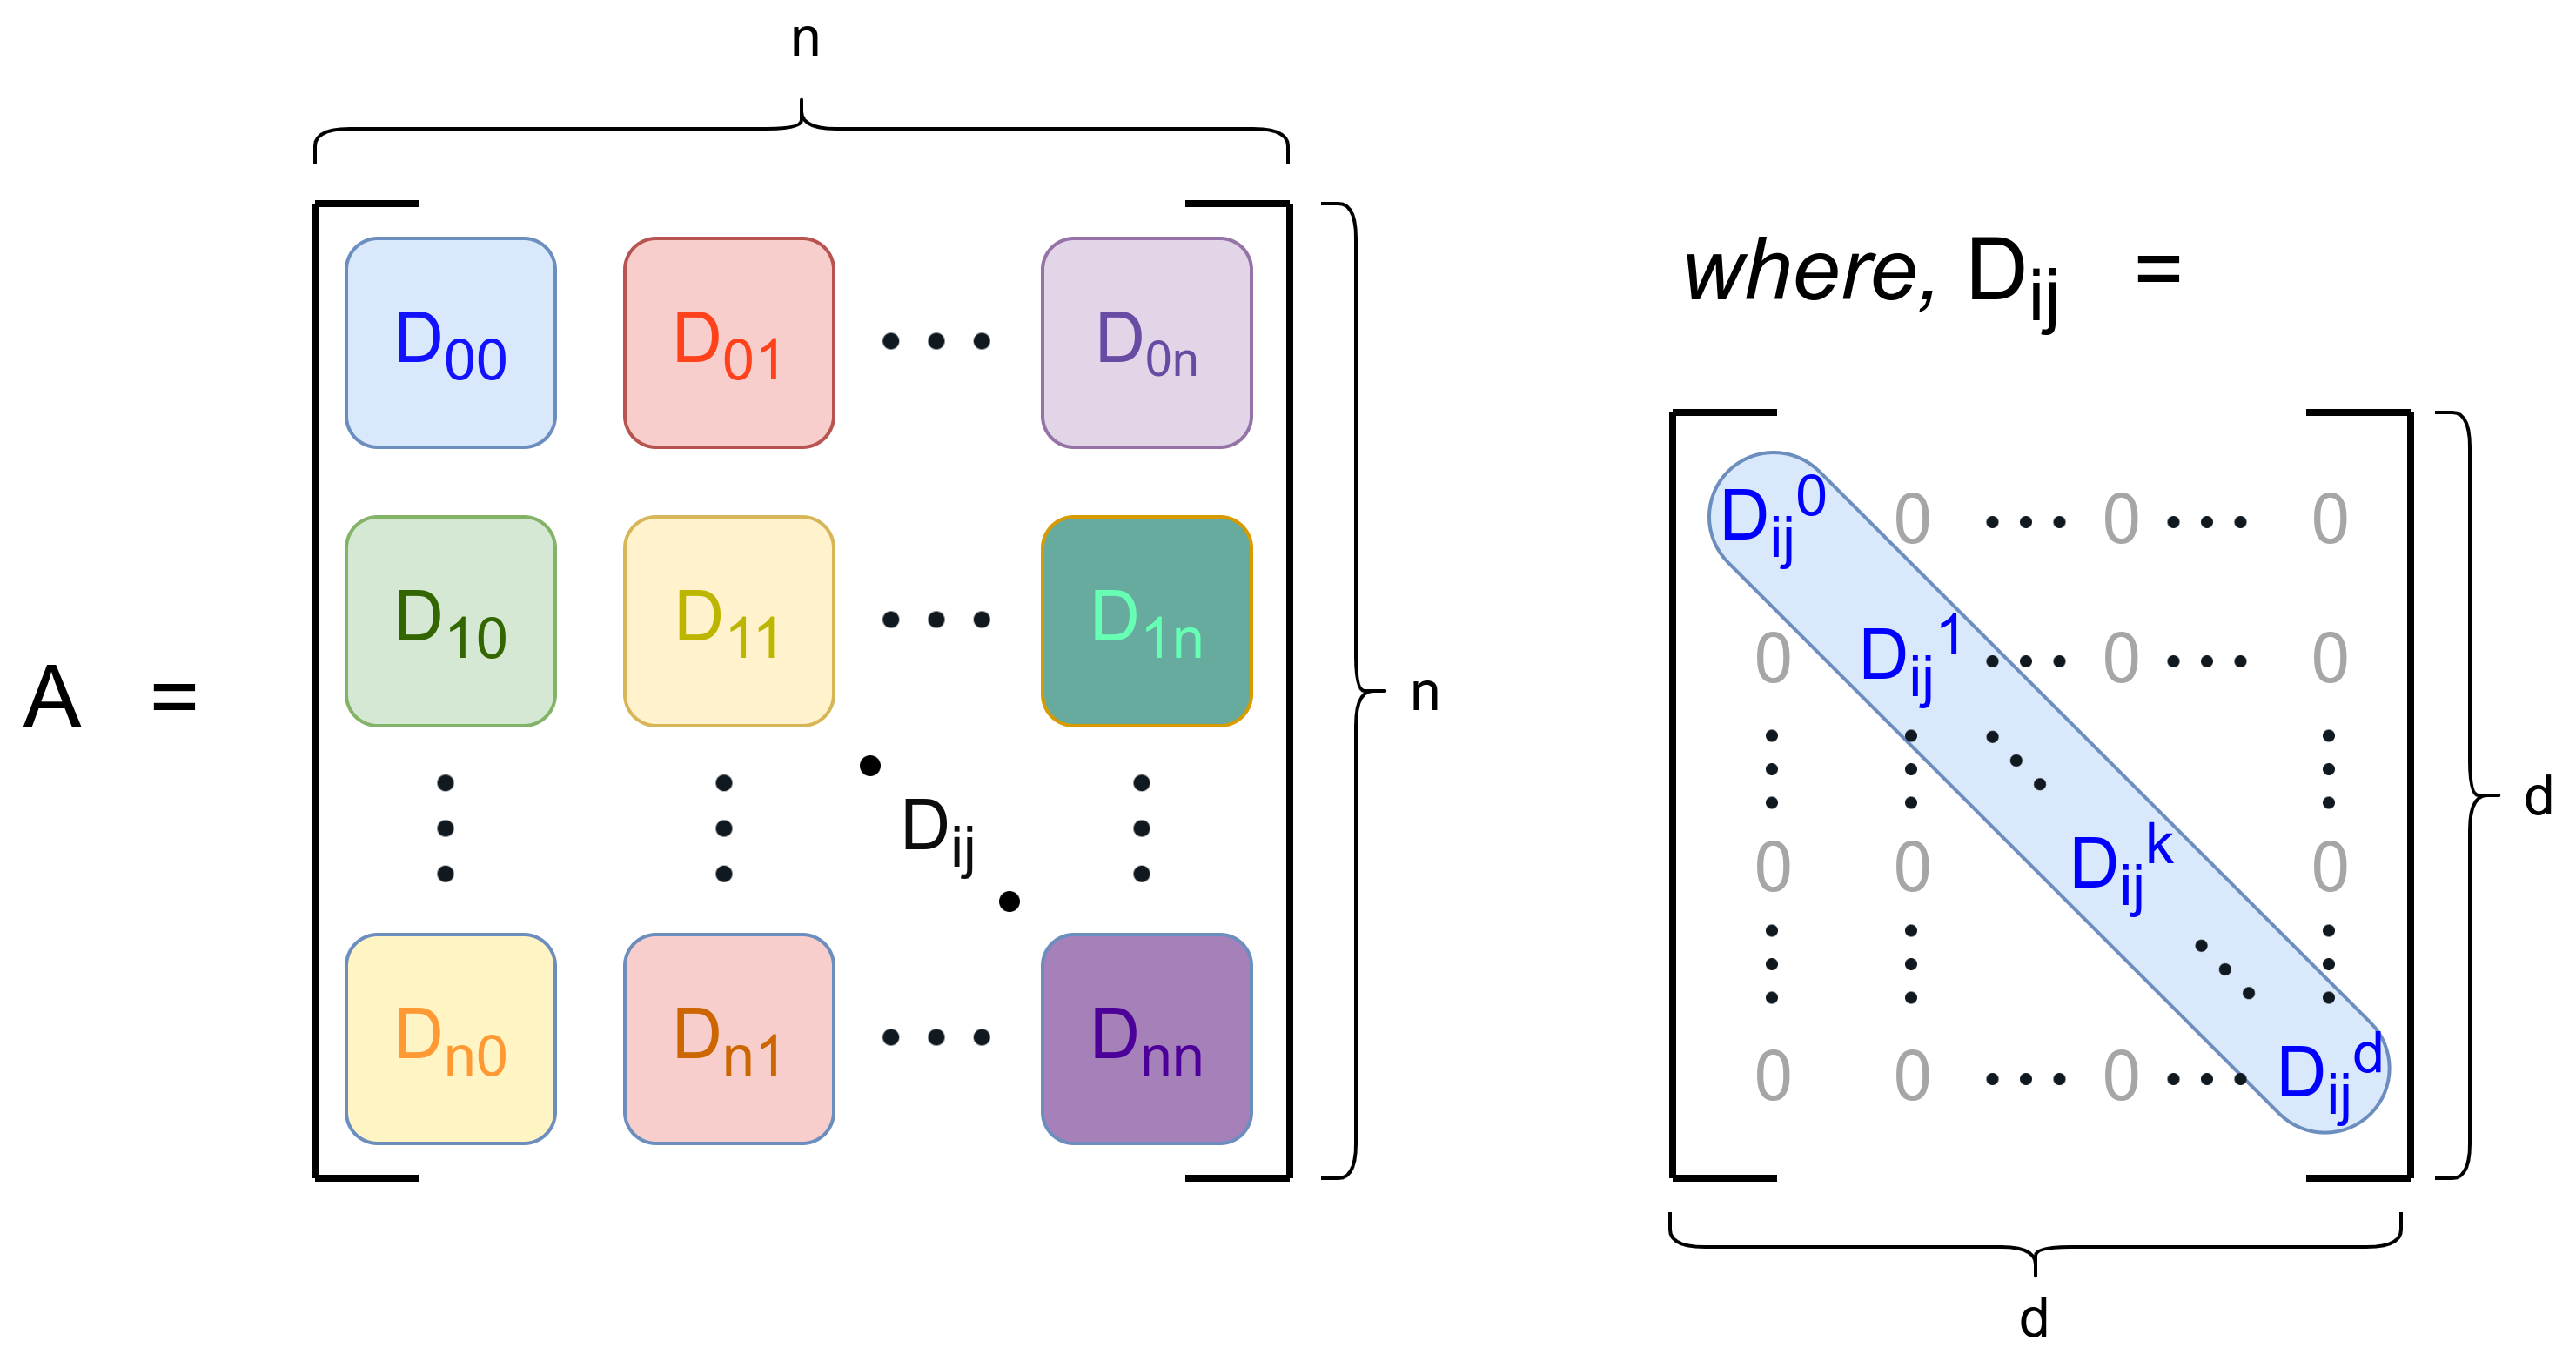
\includegraphics[width=\linewidth]{images/matrix.png}
        \caption{Matrix $A$}
        \label{img:matrix}    
    \end{figure}

    \begin{figure}[H]
        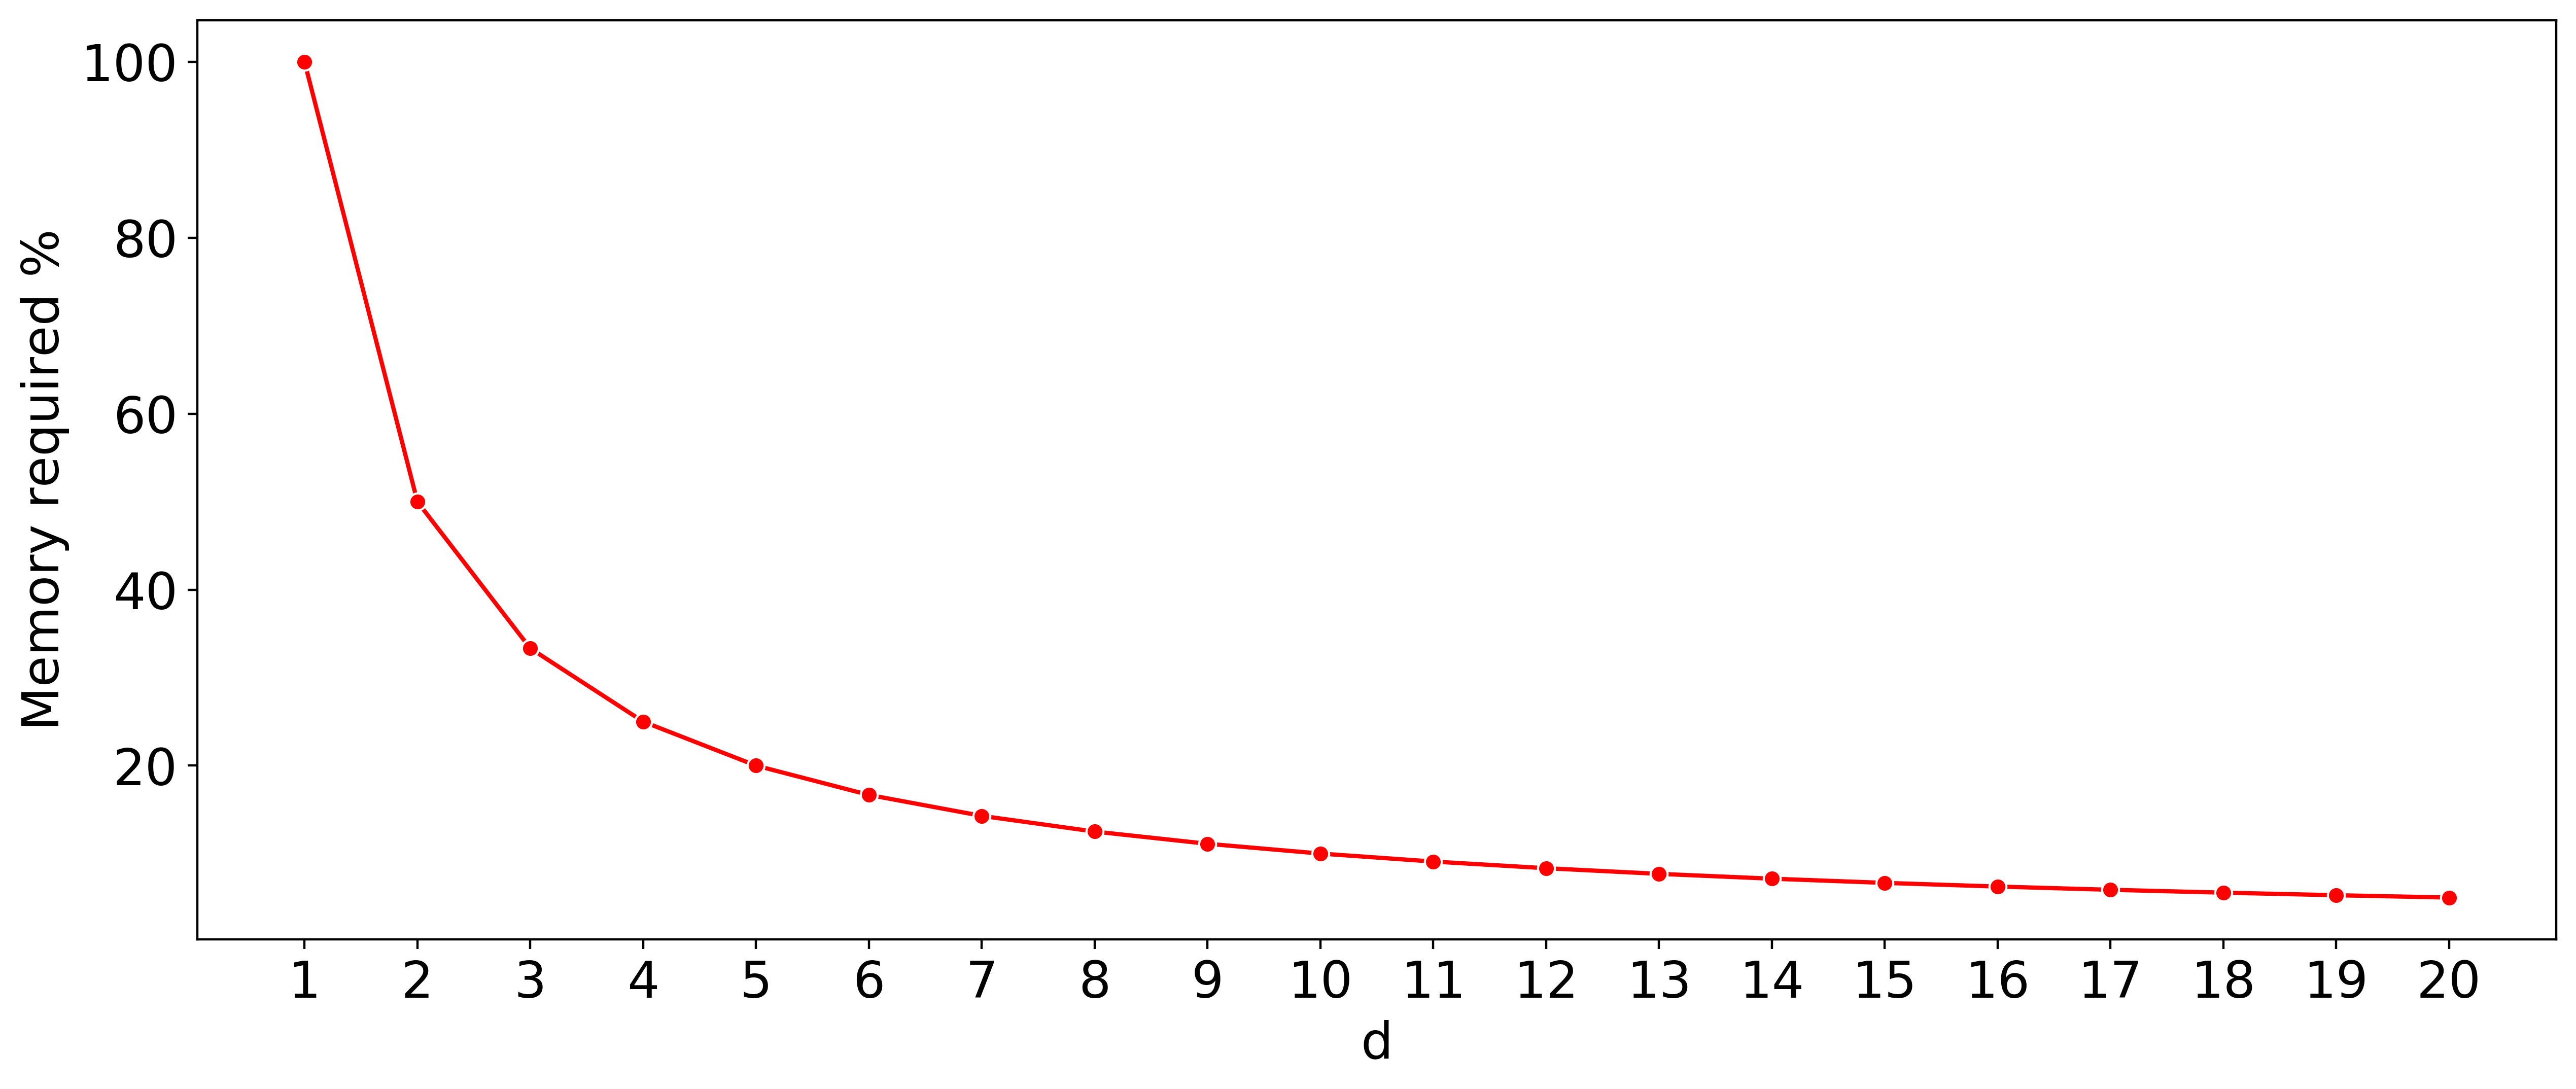
\includegraphics[width=\linewidth]{graphs/memory2.png}
        \caption{Memory Requirements of Hal Matrix (n=50)}
        \label{img:memory}    
    \end{figure}

    \Cref{img:memory} shows what percentage of memory is required if we increase $d$ and keeping $n$ constant. We can alsoalways remain same notice that when $d=1$, $100\%$ memory is required, and in this particular condition matrix is no more a sparse matrix.

    It can also be observed, that elements that are $0$, will never change after any matrix operation. So those elements can be ignored while applying matrix operation.

    The best way to store these matrices of size $\mathbb{R}^{nd \times nd}$ is to store them in an array of shape $(n^2 \times d)$ and is represented in \cref{img:representation}. Each row of the proposed data structure stores diagonal elements of the block matrix.
    
    \begin{figure}[htbp]
        \centering
        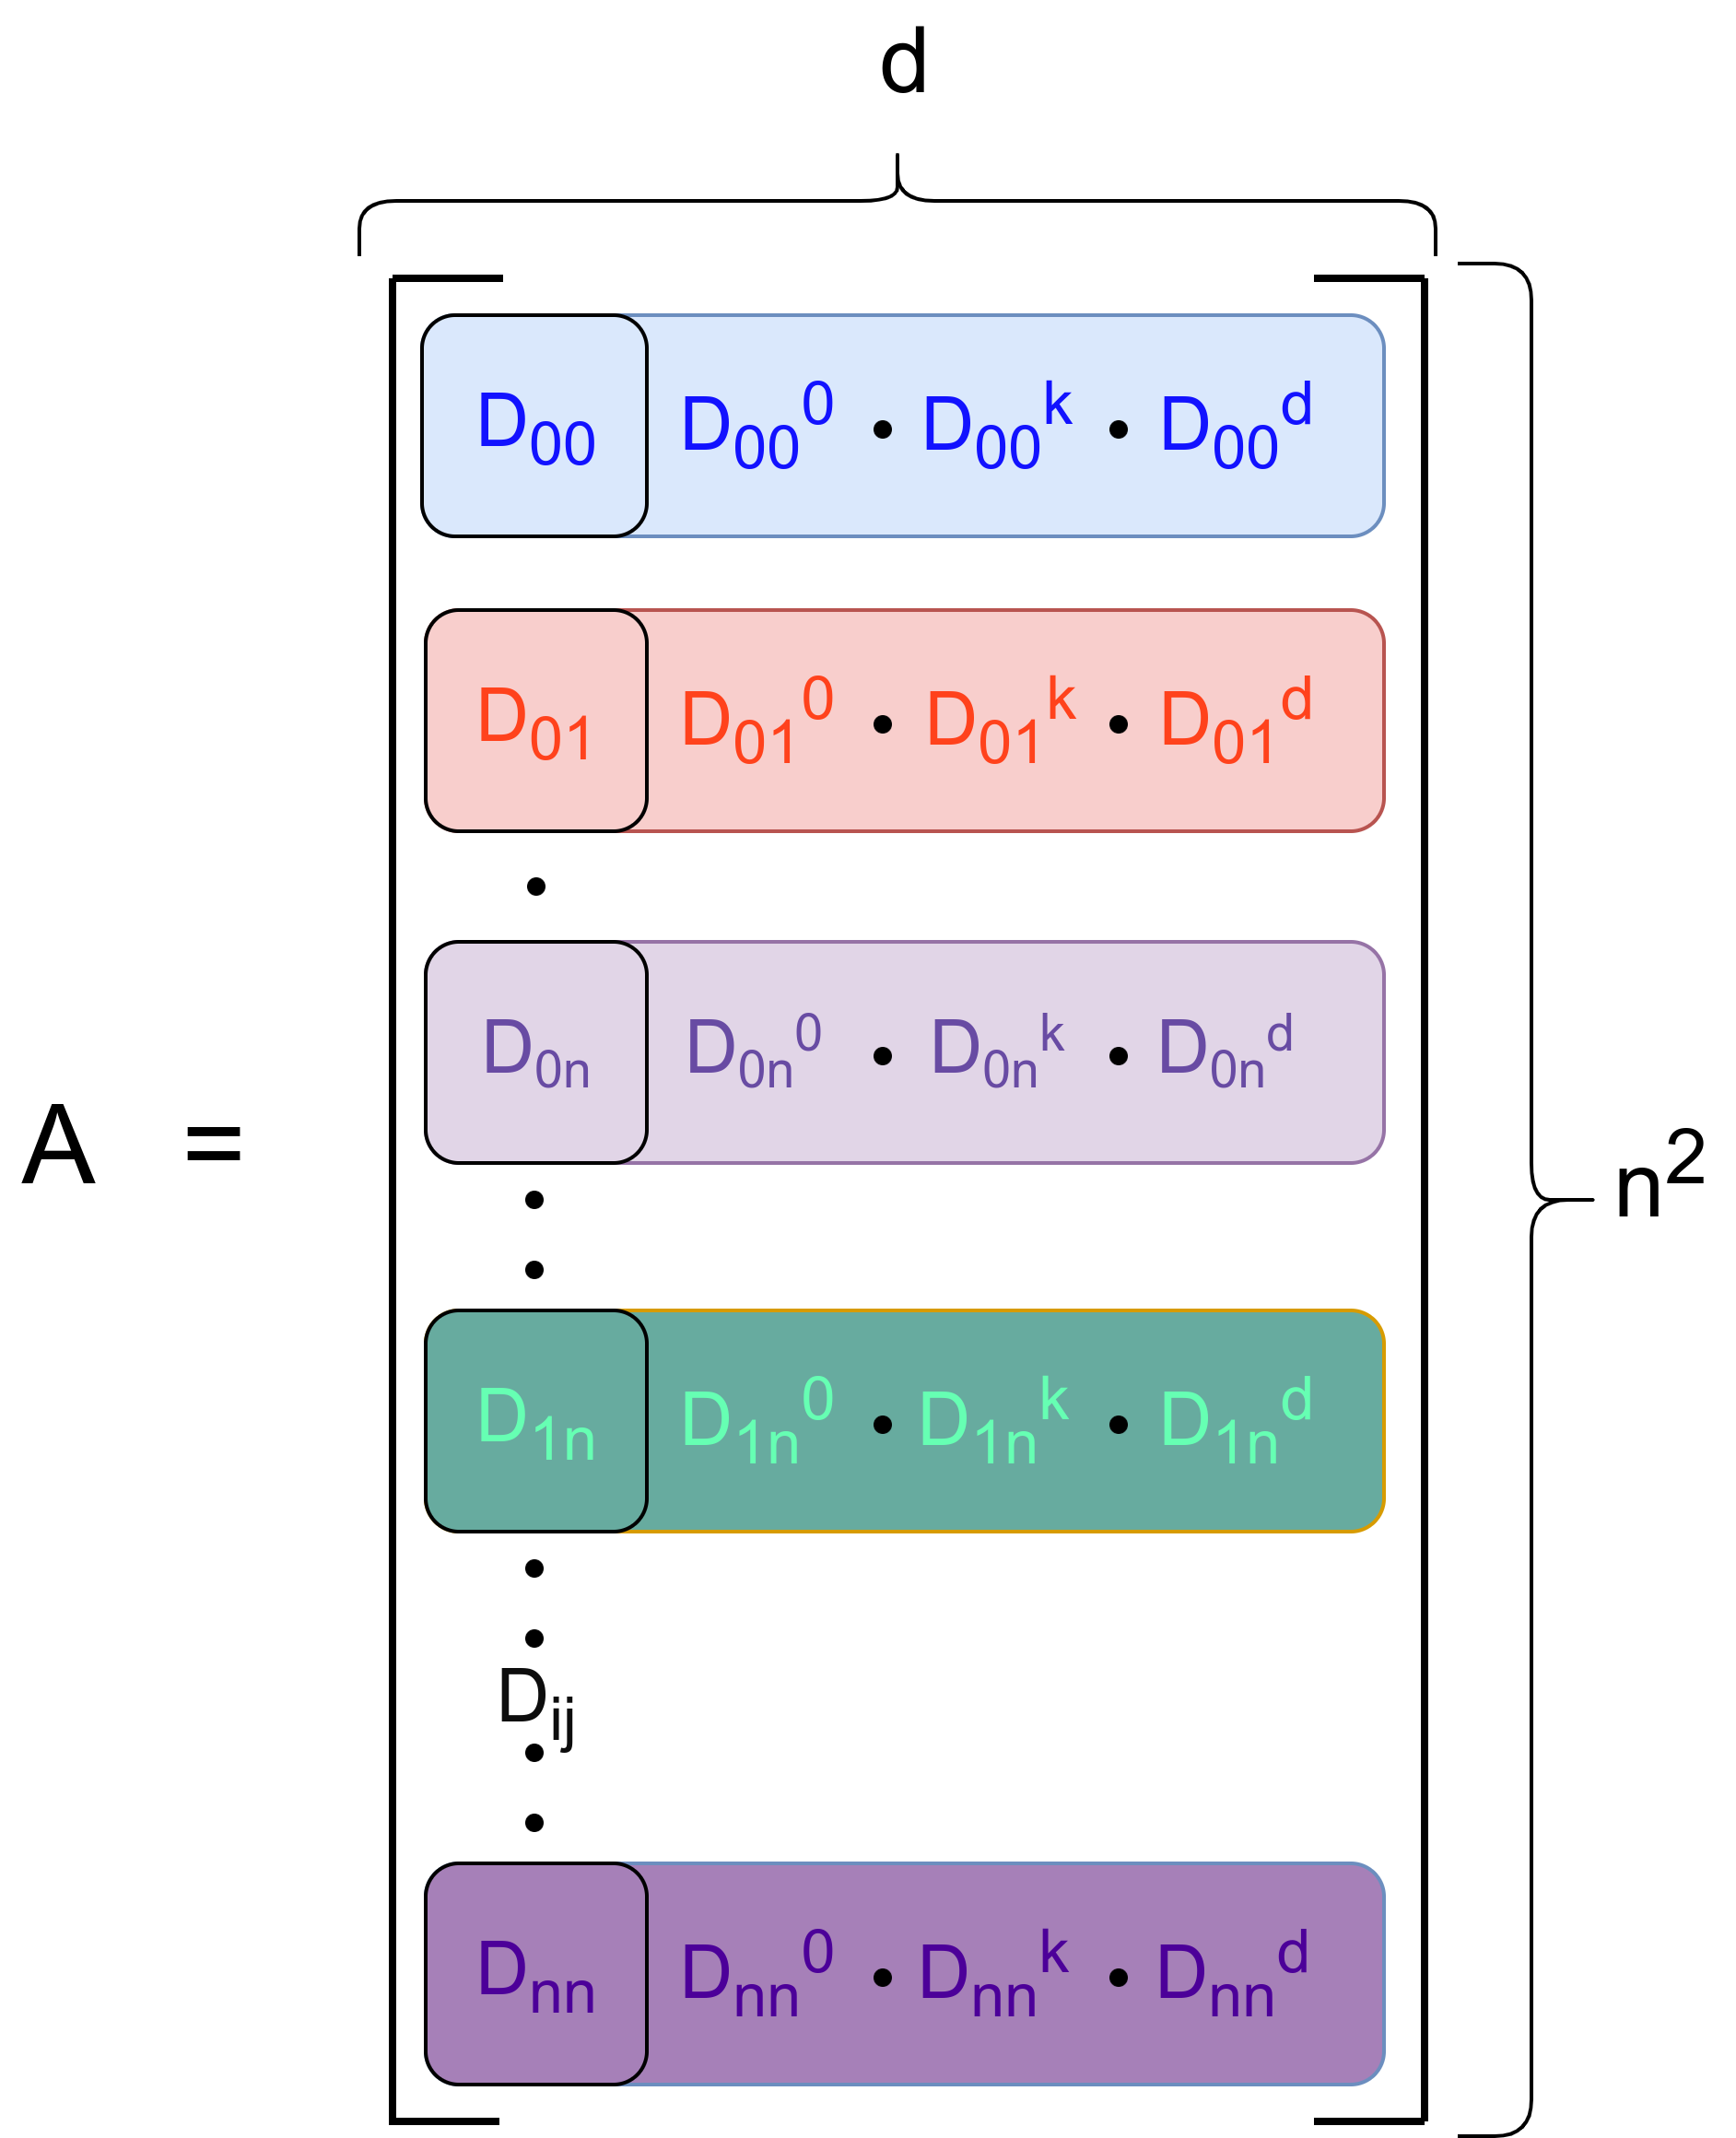
\includegraphics[width=0.8\linewidth]{images/representation.png}
        \caption{Matrix $A$ representation}
        \label{img:representation}    
    \end{figure}


\begin{figure*}[h]
    \centering
    \begin{subfigure}{0.45\textwidth}
        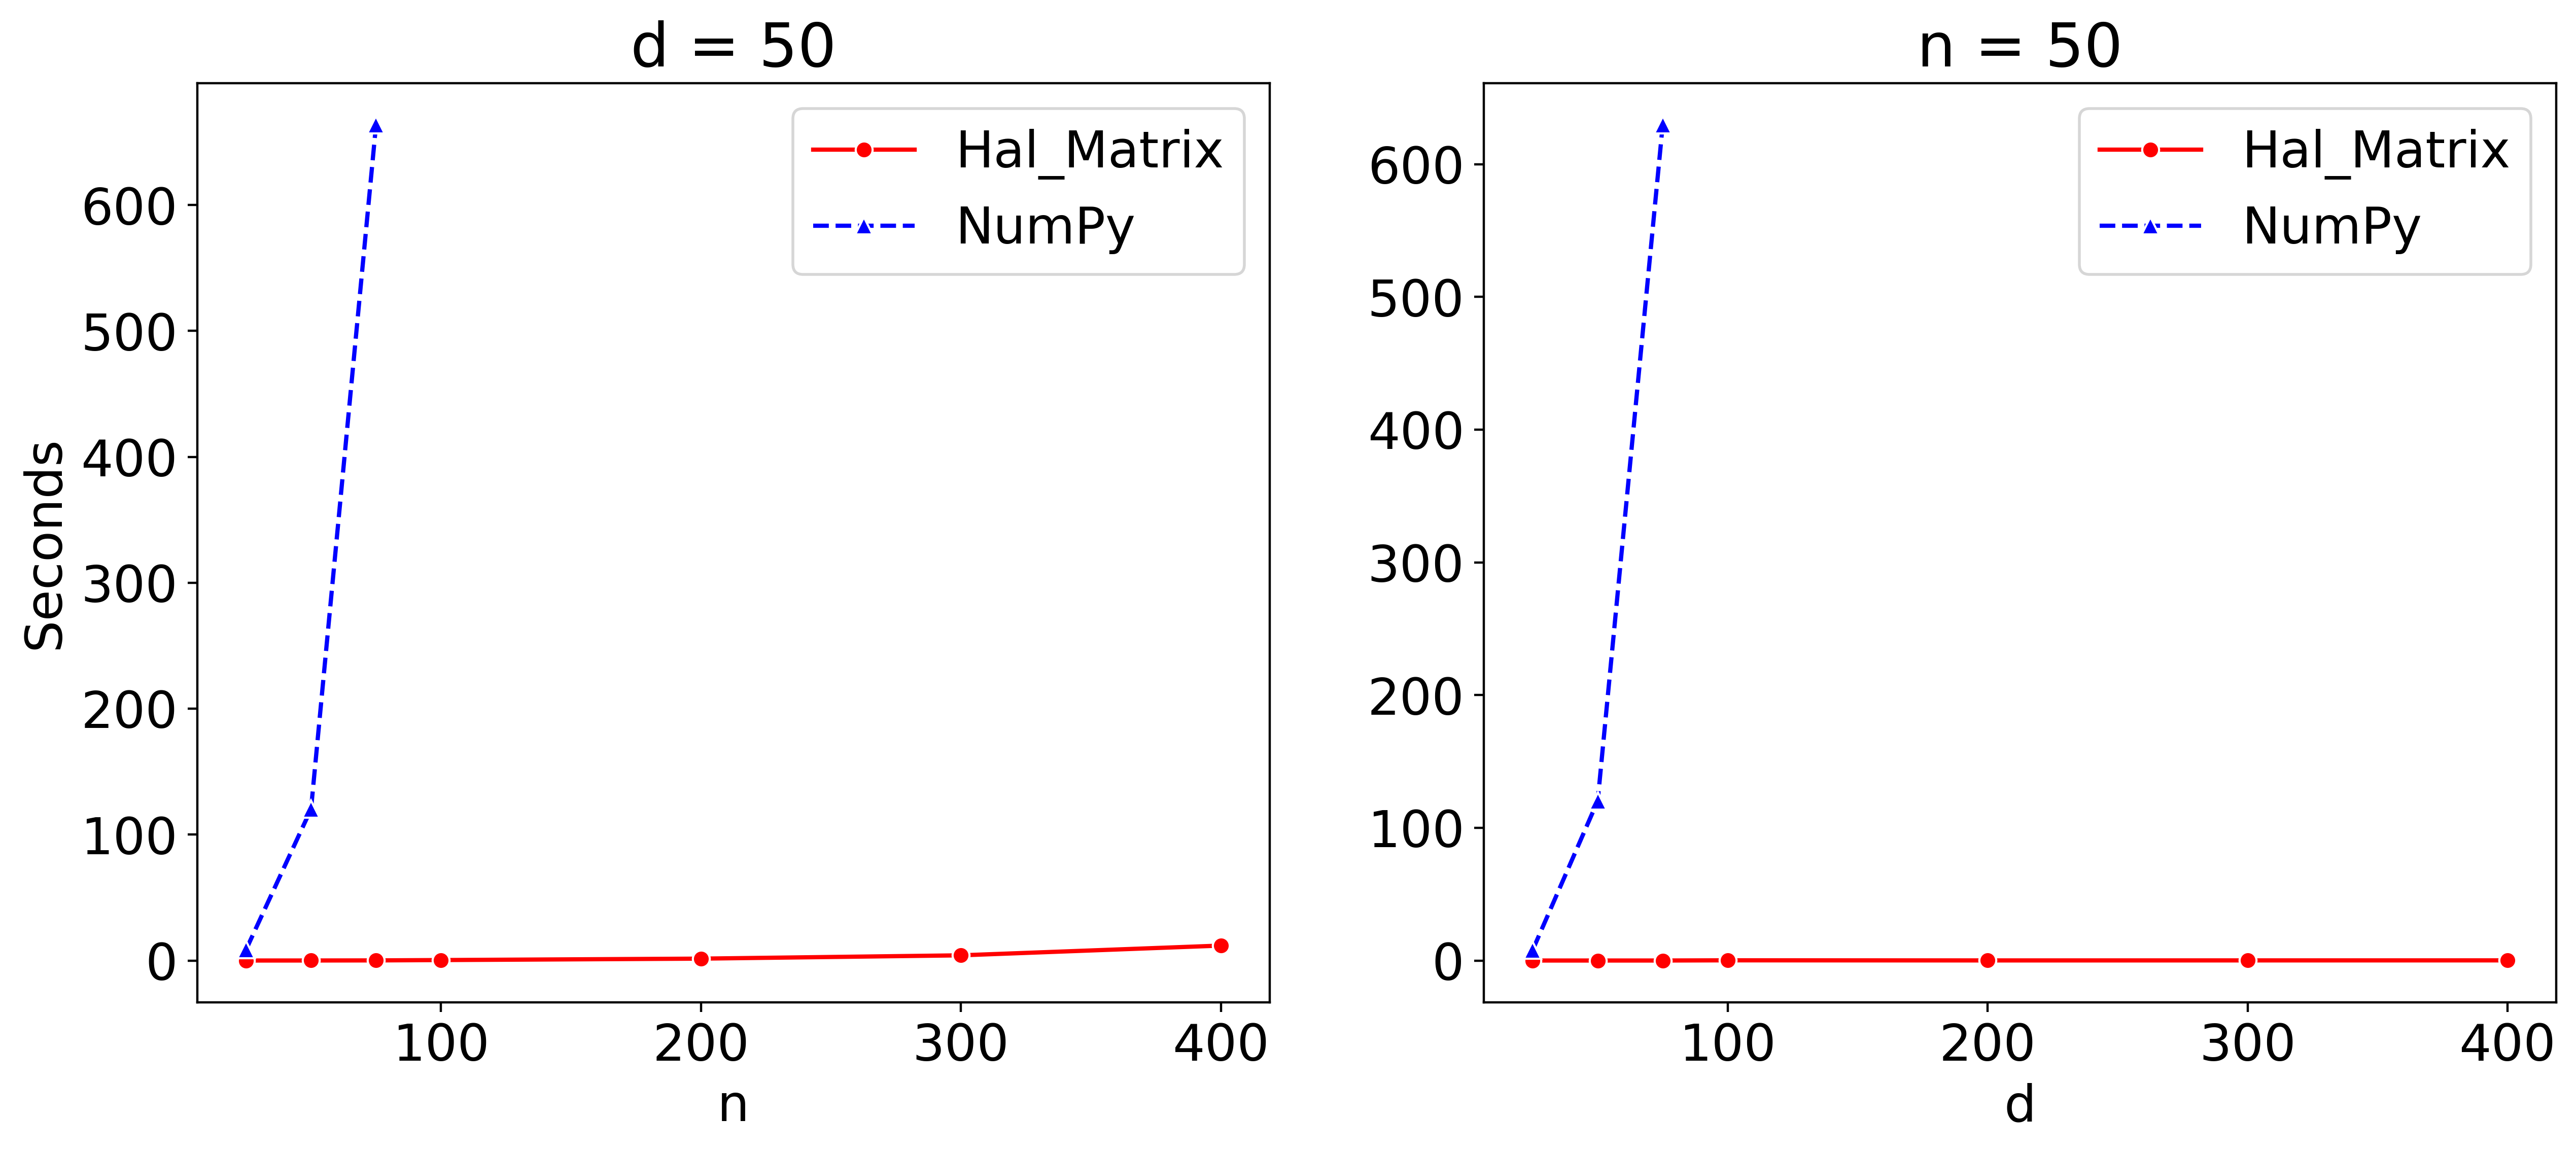
\includegraphics[width=\linewidth]{graphs/dot2.png}
        \caption{Time taken to calculate dot product (in seconds)}
        \label{img:dot}
    \end{subfigure}
    \begin{subfigure}{0.45\textwidth}
        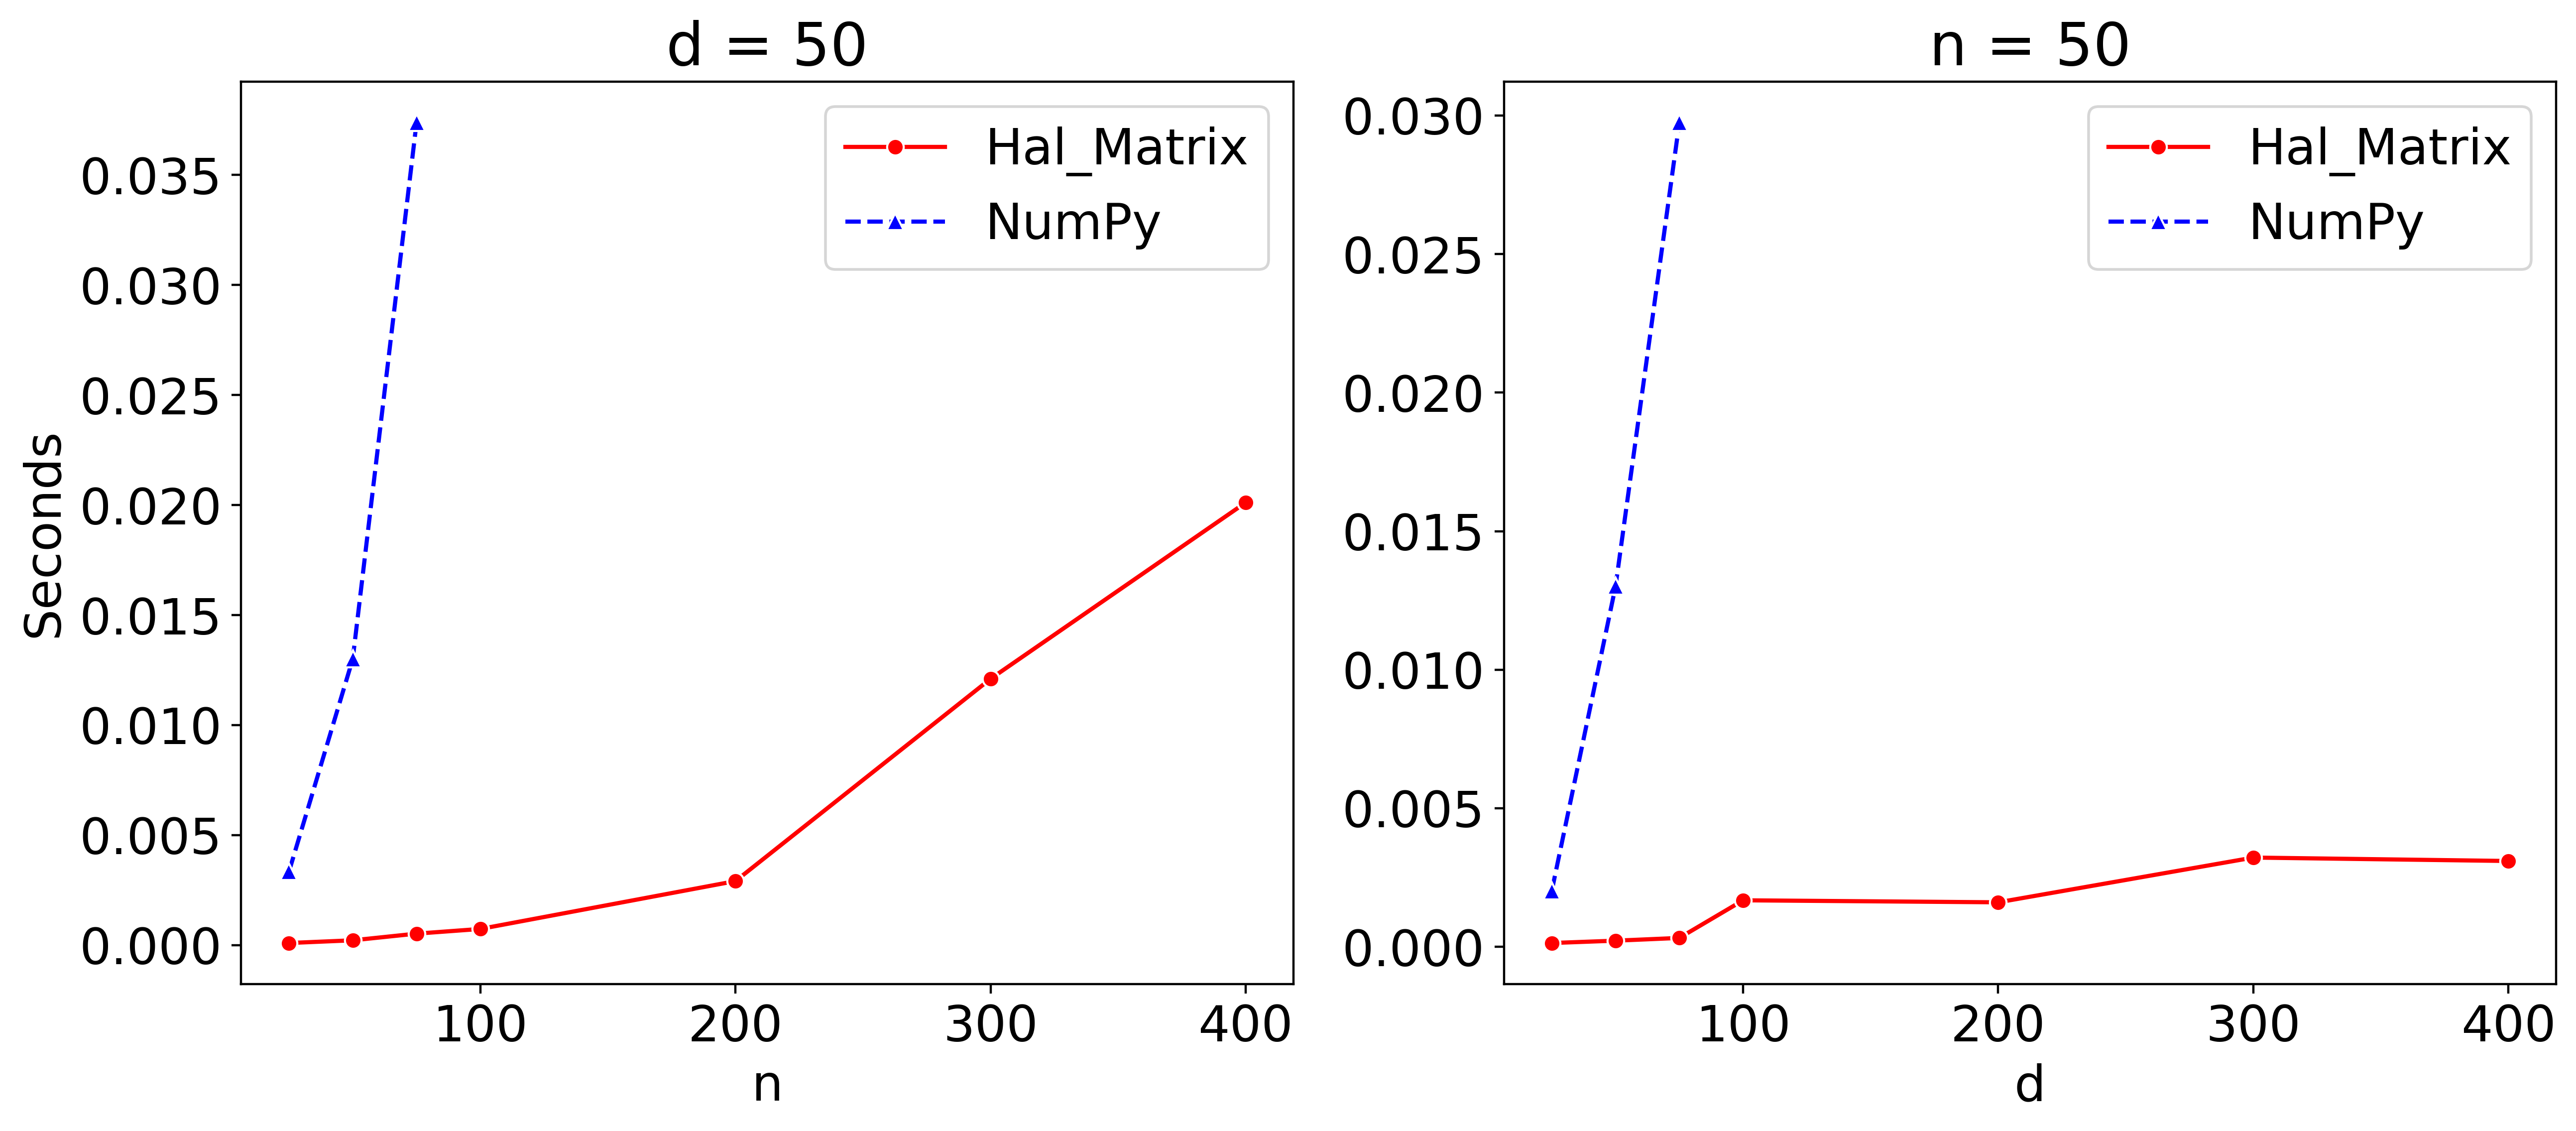
\includegraphics[width=\linewidth]{graphs/add2.png}
        \caption{Time taken to add two matrices (in seconds)}
        \label{img:add}
    \end{subfigure}
    \begin{subfigure}{0.45\textwidth}
        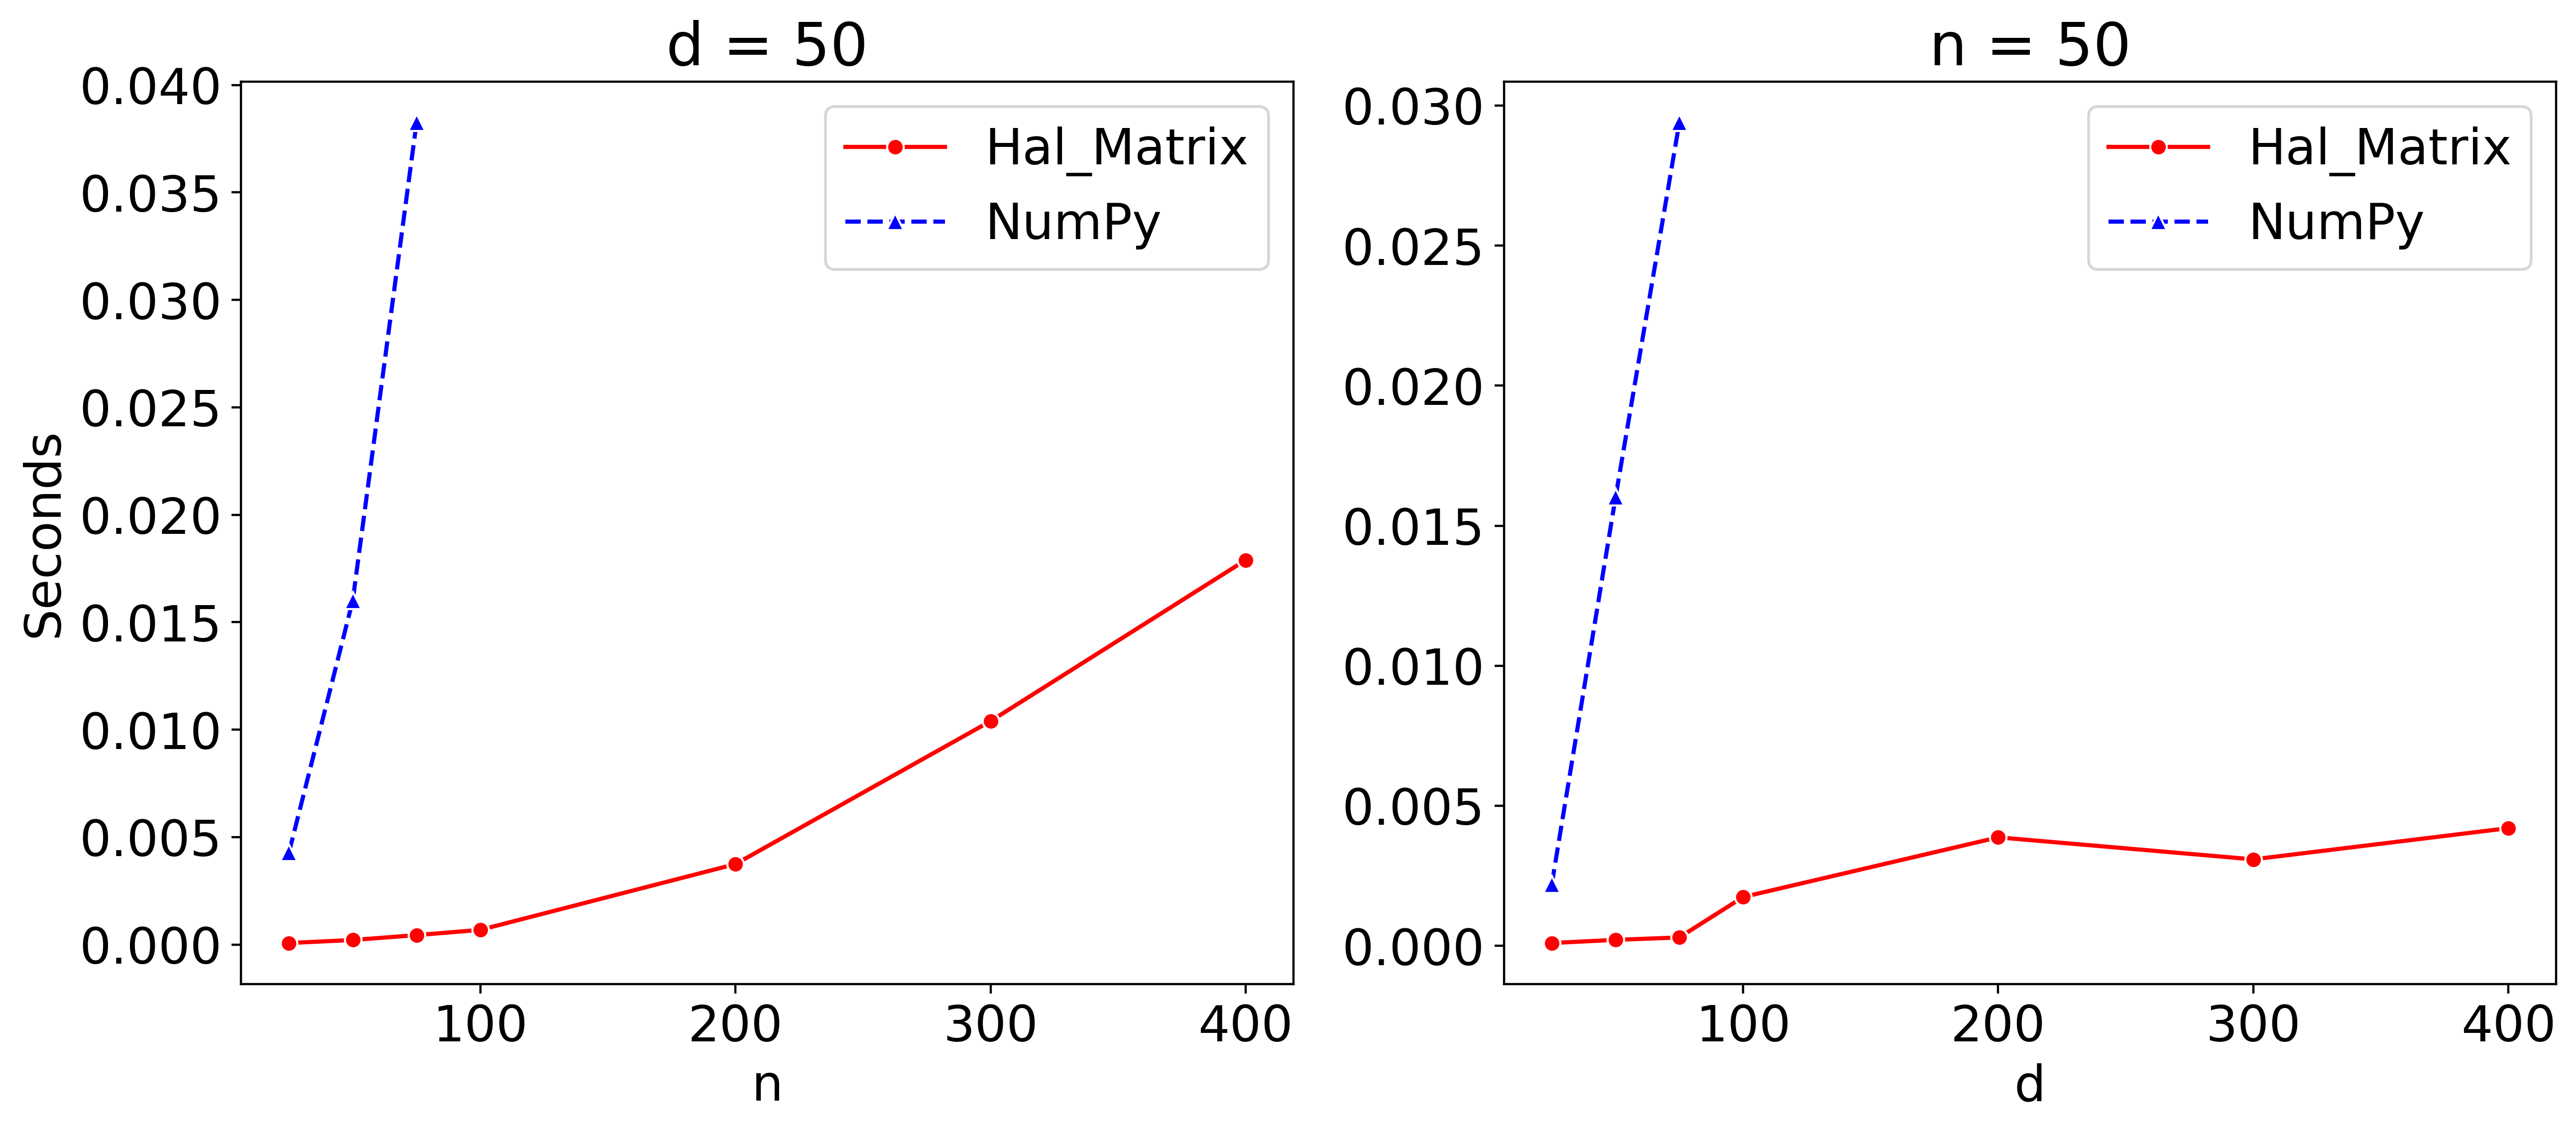
\includegraphics[width=\linewidth]{graphs/mul2.png}
        \caption{Time taken to perform element wise multiplication in two matrices (in seconds)}
        \label{img:mul}
    \end{subfigure}
    \begin{subfigure}{0.45\textwidth}
        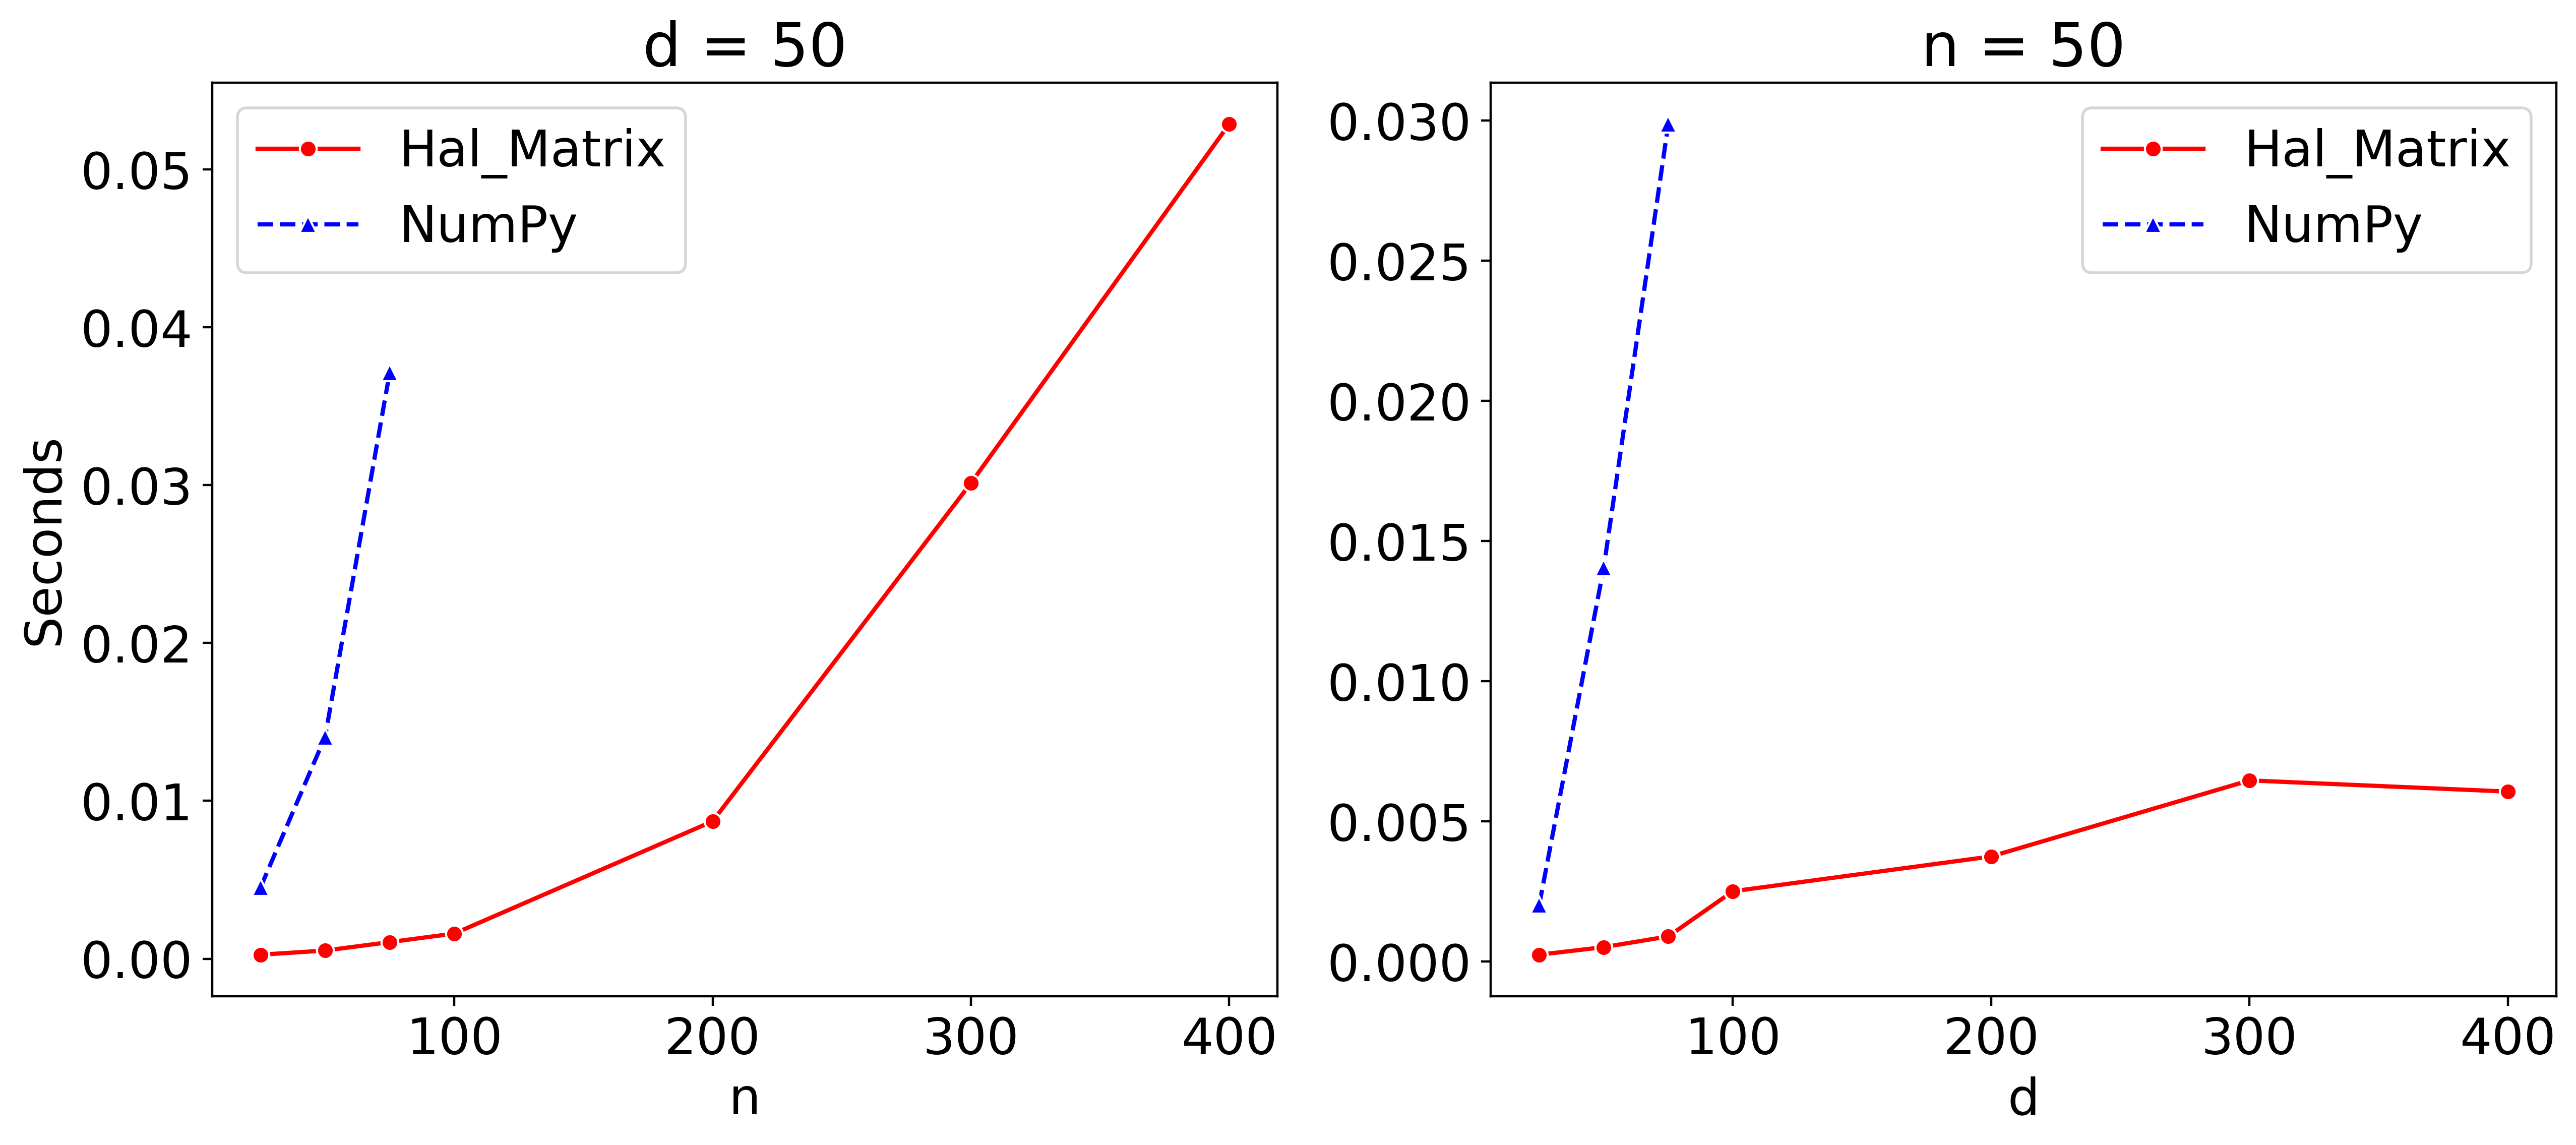
\includegraphics[width=\linewidth]{graphs/sub2.png}
        \caption{Time taken to subtract one matrix from another (in seconds)}
        \label{img:sub}
    \end{subfigure}
    \label{img:comparision}
\end{figure*}

\SetKwInOut{Input}{Input}
\SetKwInOut{Output}{Output}

\section{Matrix Operations}

    \subsection{Dot Product}

        \begin{algorithm}[!h]
            \caption{dot-product procedure}
            \SetAlgoLined
            \Input{$x$ (First Hal\_Matrix), $y$ (Second Hal\_Matrix)}
            \Output{$a$ (Output Hal\_Matrix)}

            $a$ = Hal\_Matrix($n=x.n, d=x.d$)\\
            a.data $\leftarrow$ list() \\
            \For{ i $\leftarrow$ $0$  \KwTo x.n $- 1$ }{
                left = list()\\
                \For{ k $\leftarrow i * x.n$ \KwTo $(i+1)*x.n$ }{
                    left.append(x.data[k])
                }
                \For{ j $\leftarrow$ $0$ \KwTo $x.n -1$ } {
                    right $\leftarrow$ list() \\
                    \For{ k $\leftarrow$ j \KwTo $(x.n)^{2}$, \textbf{step} $x.n$ }{
                        right.append(y.data[k])
                    }
                    res $\leftarrow$ (left * right).sum(axis=0)
                    a.append(res)
                }
            } 
        \end{algorithm}

        The above algorithm is used to find the dot product of given two matrices and \cref{img:dot} depicts the performance of the proposed data structure in comparison to NumPy arrays. NumPy arrays are fast as various operations are implemented in C language and avoid expensive "for" loops of python. The proposed data structure outperforms NumPy arrays when the matrix size is too large.
        
    \subsection{Inverse Operation}

        Gauss-Jordan Method is used to find the inverse of given hal\_matrix. The algorithm used with the proposed data structure will return the inverse of hal\_matrix if present or else it will raise NotInvertible exception.
        
    \section{Remarks}

        For complete source code of proposed data structure with algorithms checkout \href{https://github.com/rishitoshsingh/hal-matrix}{project repository}
        
        
\end{document}